\section{Methods}
\subsection{Kinematic Model}
For the analysis of differential wheelchair drive parameters using a simplified model in the reference system prorprio odometric placed in the center of the robot indicated by $RF1$. Consider that moves in a reference system fixed to the $RF0$ envoiroment.
The robot is subject to pure rolling, then we neglect slippage between wheel and ground. The angular velocities, indicated respectively with omega, are applied respectively to the right and left wheels in such a way that the components of the fixed body and the speed of the robot are related to the angular velocity of the wheels according to the equation functional (\ref{eq:velocityrelation}).
The other two support wheels are considered passive. This schematization is observable in the fig. \ref{fig:model}.
\begin{equation}
\label{eq:velocityrelation}
	\left[ \begin{array}{cc}
				v	\\									
				\omega 							
			 \end{array} 
	\right]  =\, C\,
	\left[ \begin{array}{cc}
 				\omega_\textsc{l} \\ 
				\omega_\textsc{r}
			 \end{array} 
	\right]
\end{equation}

\begin{figure}[!h]
\centering
    \resizebox{.8\linewidth}{!}{\begin{tikzpicture} [>=latex]
% \draw [help lines] (0,0) grid (8, 8);
% \foreach \x in {0,1,...,8}
%   \draw [help lines] (\x,0) node [below,%
%          font=\footnotesize] {$\x$} -- (\x,0);
%\foreach \y in {0,1,...,8}
%   \draw [help lines] (0,\y) node [left,%
%          font=\footnotesize] {$\y$} -- (0,\y);
 % body robot
 \draw [fill=lightgray, fill opacity=0.5](4, 4) circle (2.25);
 \draw [rounded corners=15,pattern=crosshatch, pattern color=gray] (0.5, 2.5)  rectangle (1.5, 5.5);
 \draw [rounded corners=15,pattern=crosshatch, pattern color=gray] (6.5, 2.5) rectangle (7.5, 5.5);
 \draw (1.5, 4) -- (6.5, 4);
 % quote wheel
 \dimline  [color=gray, 
                 %line style={thick},
                %extension start style={gray,thin},
                %extension end style={gray,thin},
               extension start length=1cm,
              extension end length=1cm,
                ]{(0, 4)}{ (0, 5.5)}{$r$};
 % quote track
 \dimline    [color=gray,
                % line style={thick},
                %extension start style={gray,thin},
                %extension end style={gray,thin},
                extension start length=-1cm,
                extension end length=-1cm
                ]{(1, 1.25)}{ (7, 1.25)}{$b$};
 % vector
 	\draw [->, blue] (4, 6) -- (4, 8) node[left]{$v$};
 	\draw [->, red] (1, 4) -- (1,7) node[left]{$\omega_{r}$};
 	\draw [->, red] (7, 4) -- (7,7)	 node[left]{$\omega_{l}$};
	\draw [->, orange] (4.75,4) arc (0:(-300+45):0.75) node[below]{$\omega$};
 % Reference system 0
 	\coordinate [label = below: \scriptsize $RF0$] (A) at (0,0);
 	\coordinate	(Bx) at	($(A)+1*(0:1)$);
 	\coordinate	(By)	at	($(A)+1*(90:1)$);
 	\draw [->] 	(A) -- (By) node[left]{$y$};
 	\draw [->] 	(A) -- (Bx) node[above]{$x$};
 % RF1
  	\coordinate [label = below: \scriptsize $RF1$] (RF1) at (4,4);
 	\coordinate	(RF1x) at	($(RF1)+1*(0:1)$);
 	\coordinate	(RF1y)	at	($(RF1)+1*(90:1)$);
 	\fill(RF1) circle (1.4pt);
 	\draw [->] (RF1) -- (RF1y) node[left] {$y'$};
 	\draw [->] (RF1) -- (RF1x) node[above] {$x'$};
 % RFcam
 	\coordinate [label = below: \scriptsize $RF_{cam}$] (R) at (4.3,2.8);
 	\coordinate (Rx) at ($(R)+1*(22.5:1)$);
 	\coordinate (Ry) at ($(R)+1*(90+22.5:1)$);
 	\fill (R) circle (1.4pt);
	 \draw [->, darkgray] (R) -- (Ry) node[left] {$y_{cam}$};
 	 \draw [->, darkgray] (R) -- (Rx) node[above]{$x_{cam}$};
 \end{tikzpicture}}
\caption{Robot kinemati model}
\label{fig:model}
\end{figure}
\noindent Where the matrix $\textbf{C} \in \RealNumber^{2 x 2}$ is defined as (\ref{eq:Cmatrix}):
\begin{equation}
\label{eq:Cmatrix}
	\left[ \begin{array}{cc}
 				\frac{r_\textsc{r}}{2} &	\frac{r_\textsc{l}}{2} \\
				\frac{r_\textsc{l}}{b} &	-\frac{r_\textsc{l}}{b} 
			 \end{array} 
	\right]
\end{equation}
in which $r_\textsc{r}$ and $r_\textsc{l}$ are the radii of the right and left wheel, respectively.
The odometry of a vehicle is usually implemented by discrete-time integration, such as (\ref{eq:odometry}):
\begin{equation}
\label{eq:odometry}
	\begin{cases}
		x_{k+1} = x_{k} + T \, v_{k} \, cos(\theta_{k} + T \,\omega_{k}/2)\\
		y_{k+1} = y_{k} + T \, v_{k} \, sin(\theta_{k} + T \, \omega_{k}/2)\\
		\theta_{k+1} = \theta_{k} + T \, \omega_{k}
	\end{cases}
\end{equation}           
Notice that low sampling frequency and high vehicle velocities can be a significant source of odometric error.
\subsection{Data Analysis}
To achieve the objective of calibration of the geometric parameters of the robot there were provided four datasets where in each of which collected the information from the camera and from the incremental encoder.
First data operation was carried out by a python script to correct the angle sign registered as evaluated with a negative sign.
Second operation and change the left encoder incremental measuring as being mounted on reverse respect to the right its value must be taken with a negative sign.
In the file is observed the possibility of the presence of two successive rows with the same timestamp. This means that at the same time have been changed both the encoder ticks and the camera pose or covariance.
It may be noted that in one line has changed the camera information and the other the odometer ticks. Thus, at the same timestamp, in the second row is the information are modified.
So you chose to eliminate duplicate rows preserve the last where both information camera pose or covariance and ticks has changed.
To achieve this, it is made use of the possibilities offered by data structures provided by Python fact realizing a dictionary between camera pose values and covariance, so it was possible to compare multiple values at the same instant and eliminate redundant data.
\subsection{Calibration Techinque}
To estimate the parameters of the robot expressed in the equation (\ref{eq:Cmatrix}), namely, the wheel radius values indicated with "$r_\textsc{r}$" and "$r_\textsc{l}$", and the axle track as indicated "$b$", using the method described in the report \cite{1512356}.
Experiments of odometry calibration require measurement of the absolute position and orientation of the mobile robot at suitable locations along the motion trajectories. For instance this calibration technique requires measurement of the starting and final robot configuration for each motion execution. The datasets supplied information related to: the camera position $x, y, \theta$ and increments of the encoder. Each information is saved in columns: 
\begin{itemize}
\item column 1: acquisistions time [ms];
\item columns 2--3--4: camera pose $x, y, \theta$ [cm, cm, rad];
\item column from 5 to 13: camera covariance ordered by rows [cm$^2$] for pose, [rad$^2$] for angle and [cm*rad] for mixed terms ;
\item colunm 14--15: odometric Encoder ticks Left and Right;
\end{itemize}
It has been chosen to perform the odometry calibration whereas in the same calculation all four datasets provided as suggested by the technique used. Then the equations (\ref{eq:Phi4}) and (\ref{eq:XY4}) are rewritten limited to the four paths to obtain:
\begin{equation}
\label{eq:Phi4}
	\begin{bmatrix}
		\hat{c}_{2,1}\\
		\hat{c}_{2,2}
	\end{bmatrix} =	(\bar{\Phi}_{\theta}^{\textsc{t}} \, \bar{\Phi}_{\theta})^{-1} \, \bar{\Phi}_{\theta}^{\textsc{t}} \, 
	\begin{bmatrix}
		\theta_{\textsc{n},1} - \theta_{\textsc{n},0}\\
		\theta_{\textsc{n},2} - \theta_{\textsc{n},0}\\
		\theta_{\textsc{n},3} - \theta_{\textsc{n},0}\\
		\theta_{\textsc{n},4} - \theta_{\textsc{n},0}
	\end{bmatrix}
\end{equation}
\begin{equation}
\label{eq:XY4}
	\begin{bmatrix}
		\hat{c}_{1,1}\\
		\hat{c}_{1,2}
	\end{bmatrix} = (\bar{\Phi}_{xy}^{\textsc{t}} \, \bar{\Phi}_{xy})^{-1} \, \bar{\Phi}_{xy}^{\textsc{t}} \, 
	\begin{bmatrix}
		xy_{\textsc{n},1} - xy_{\textsc{n},0}\\
		xy_{\textsc{n},2} - xy_{\textsc{n},0}\\
		xy_{\textsc{n},3} - xy_{\textsc{n},0}\\
		xy_{\textsc{n},4} - xy_{\textsc{n},0}
	\end{bmatrix}
\end{equation}
 As a result of simulations shows the values of the matrix C:
\begin{equation}
\label{eq:Cresult}
	\begin{bmatrix}
		8.1873  &  6.5229\\
    	0.2823 &  -0.2807
	\end{bmatrix}
\end{equation}
It is noted that the parameters $c_ {1,1}$ and $c_ {1,2}$ relative to the spokes of the wheels are different from each other, this is due to the simplifications introduced by the kinematic model. On the other hands, the axle values $c_ {2,1}$ and $c_ {2,2}$, without the negative sign, are much more similar because precedenemente estimated at $c_{1,j}$ and therefore do not contain the error propagation.
Subsequently, it calculates the average between the values of the obtained rays and the standard deviation, these are shown in the table (\ref{tab:recapvalue}).
\begin{table}[!h]
\centering
	\begin{tabular}{lccc}
		\hline
								& Radius 	& Mean 	& standard  \\
								&	[mm]	& [mm]	& deviation [mm]\\
		\hline
		$r_\textsc{r}$	&	$130.457$		& $147.102	$		&	$\pm23.538$\\
		$r_\textsc{l}$	&	$163.746$		& $147.102	$		&	$\pm23.538$\\
		$b$					&	$522.43$\\
		\hline
\end{tabular}
\caption{estimated value}
\label{tab:recapvalue}
\end{table}
%
%\begin{figure*}[htb]
%\subfloat[][\emph{dataset 1}.]
%   {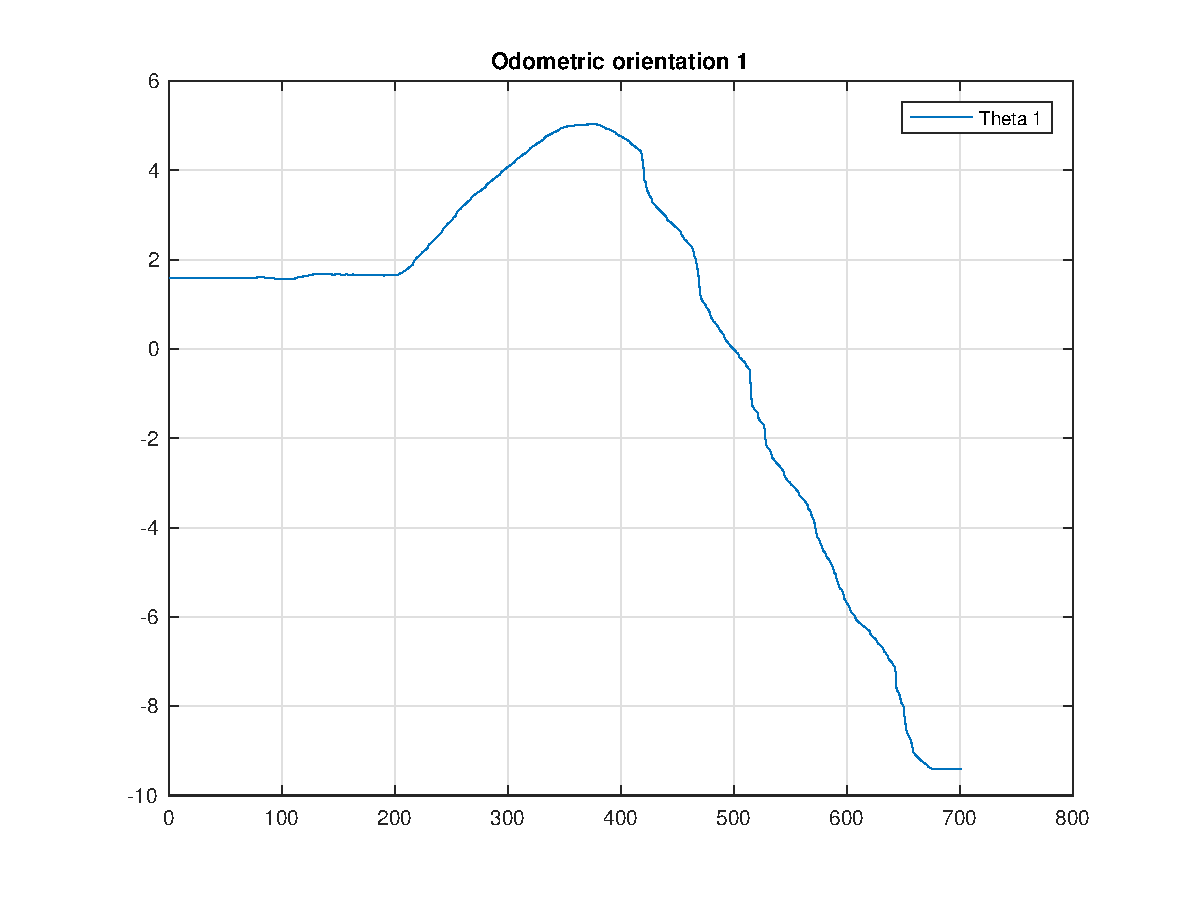
\includegraphics[width=.30\textwidth]{angle_dataset_1.eps}} \,
%\subfloat[][\emph{dataset 2}.]
%   {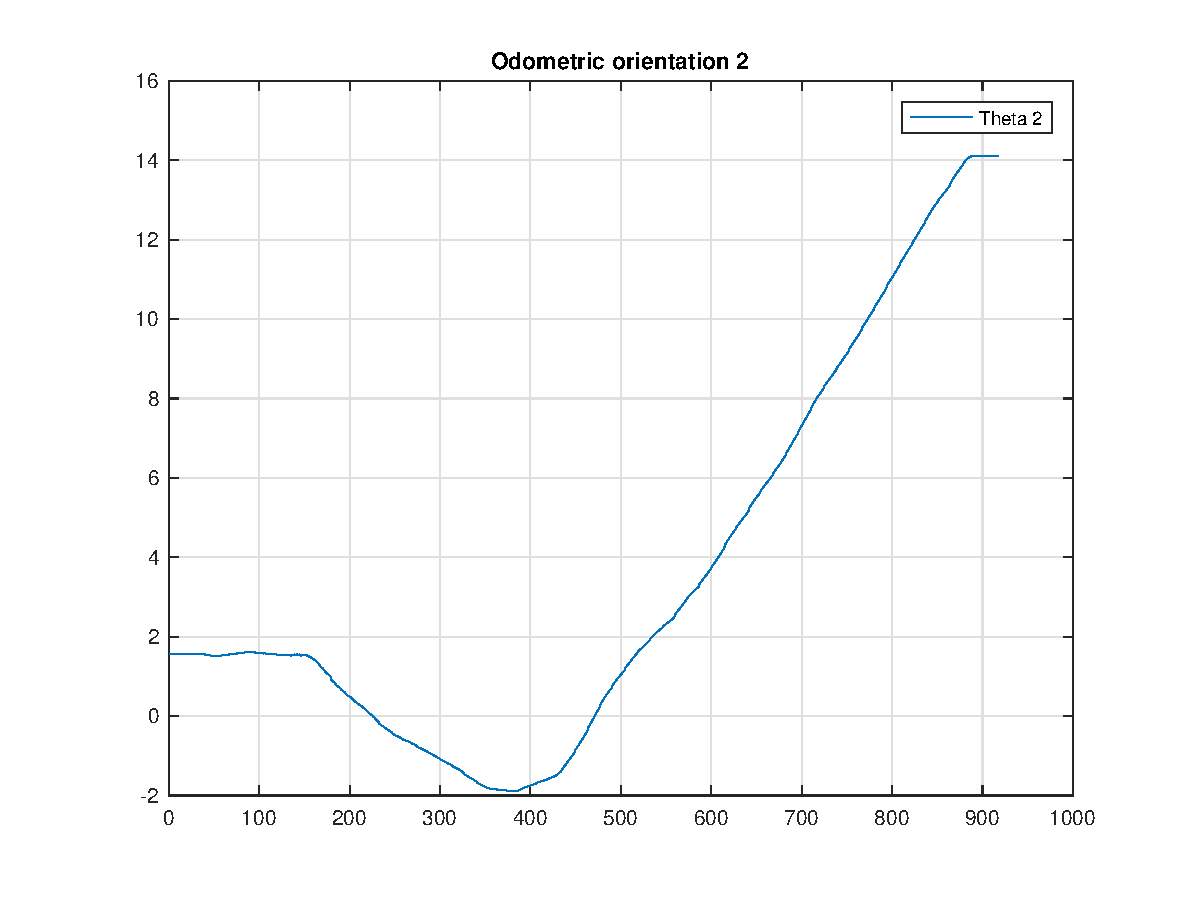
\includegraphics[width=.30\textwidth]{angle_dataset_2.eps}} \,
%\subfloat[][\emph{dataset 3}.]
%   {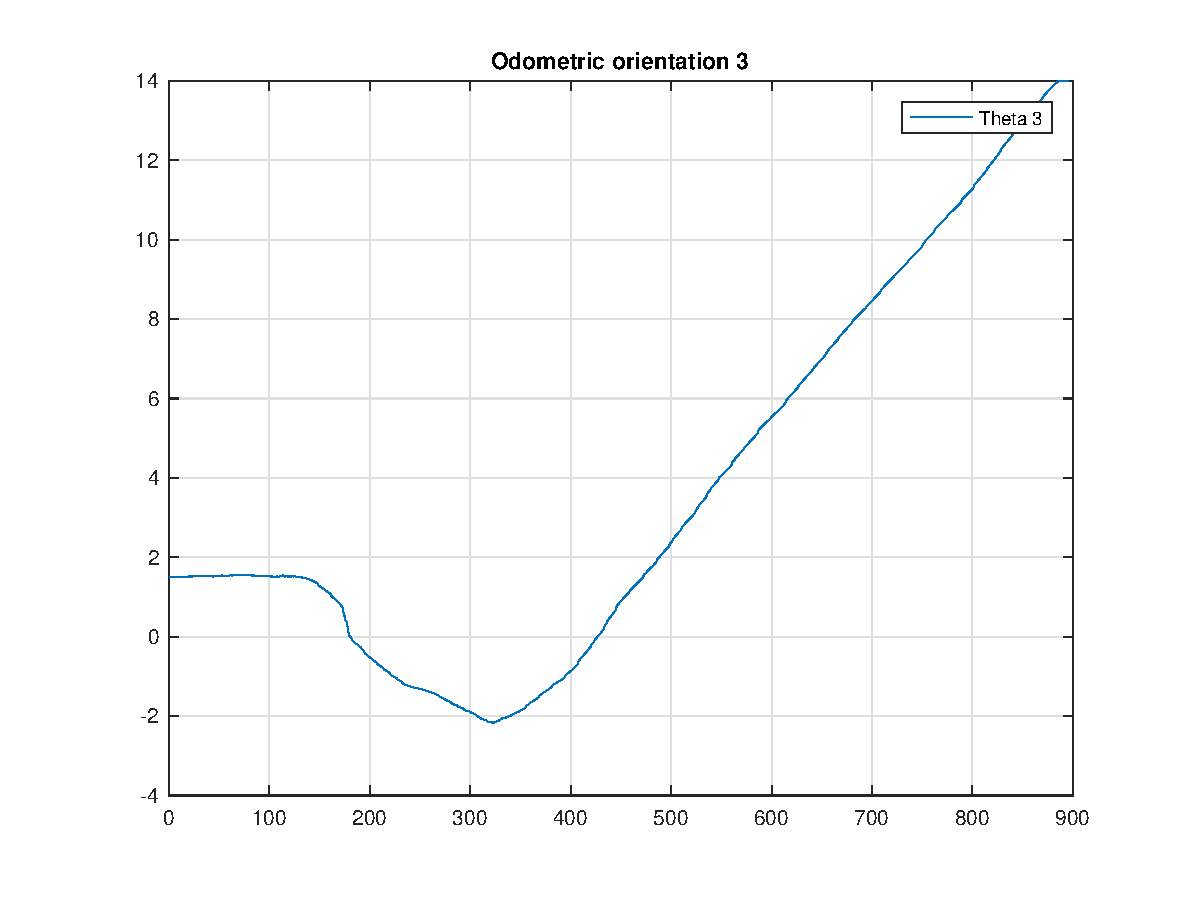
\includegraphics[width=.30\textwidth]{angle_dataset_3.eps}} \,
%\subfloat[][\emph{dataset 4}.]
%   {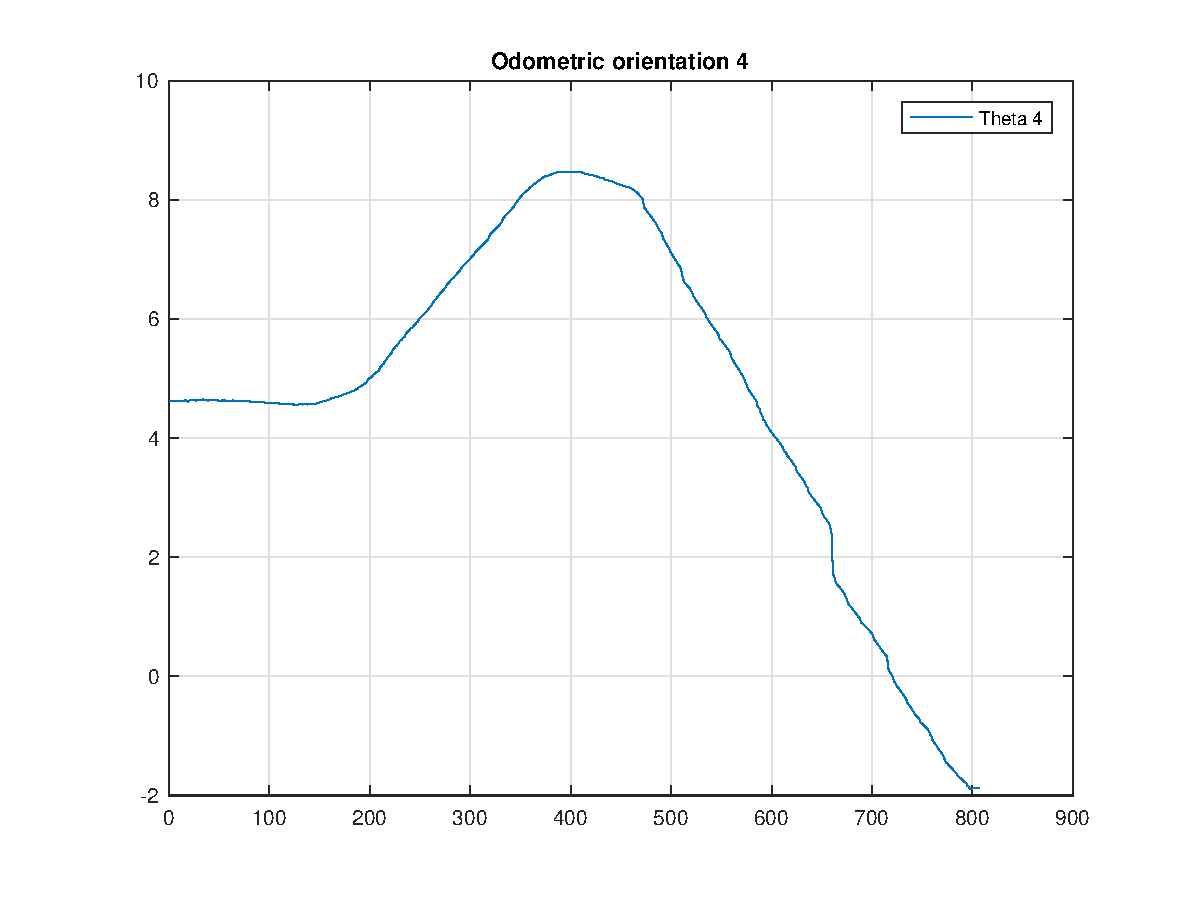
\includegraphics[width=.35\textwidth]{angle_dataset_4.eps}}\\
%%\caption{Angle captured by the camera}
%\end{figure*}
%
%\begin{figure*}[htb]
%\subfloat[][\emph{dataset 1}.]
%   {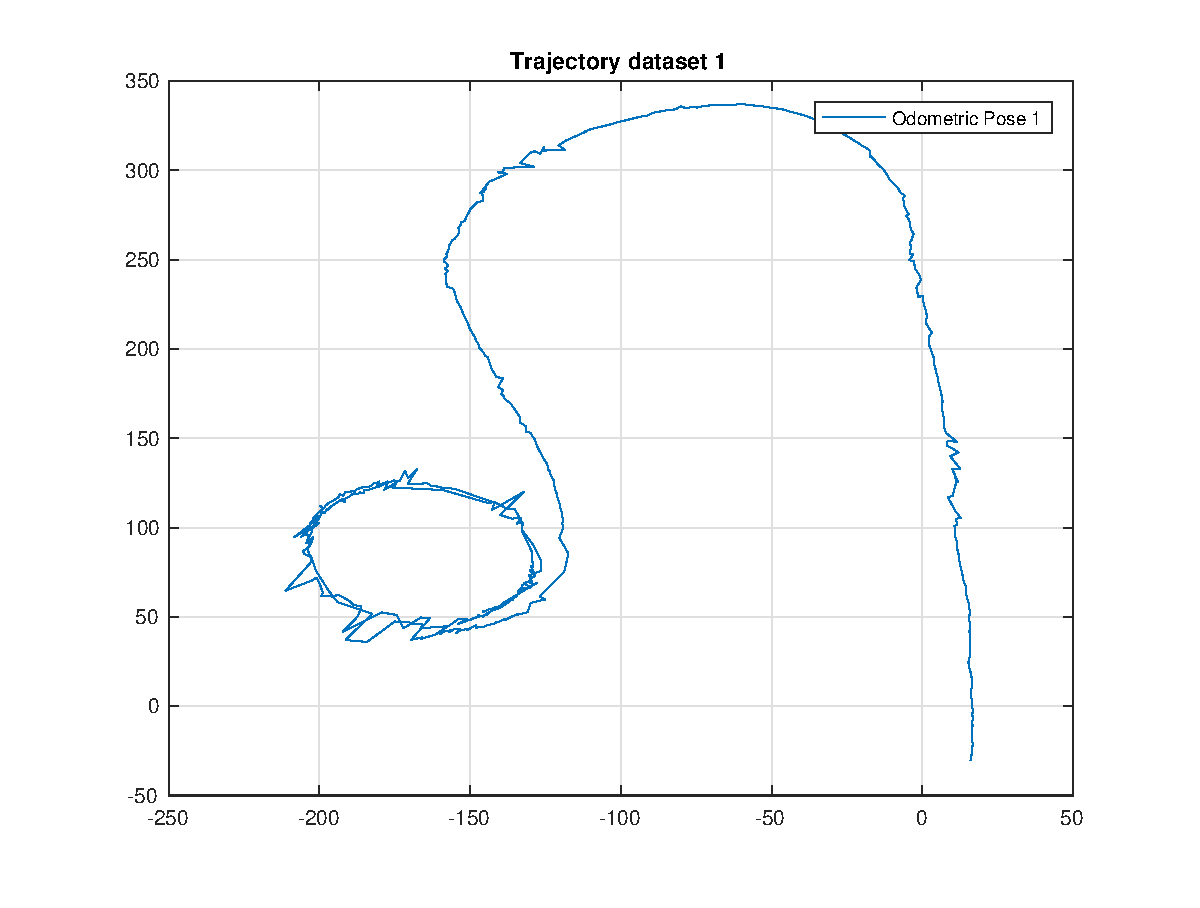
\includegraphics[width=.35\textwidth]{trajectory_dataset_1.eps}} \,
%\subfloat[][\emph{dataset 2}.]
%   {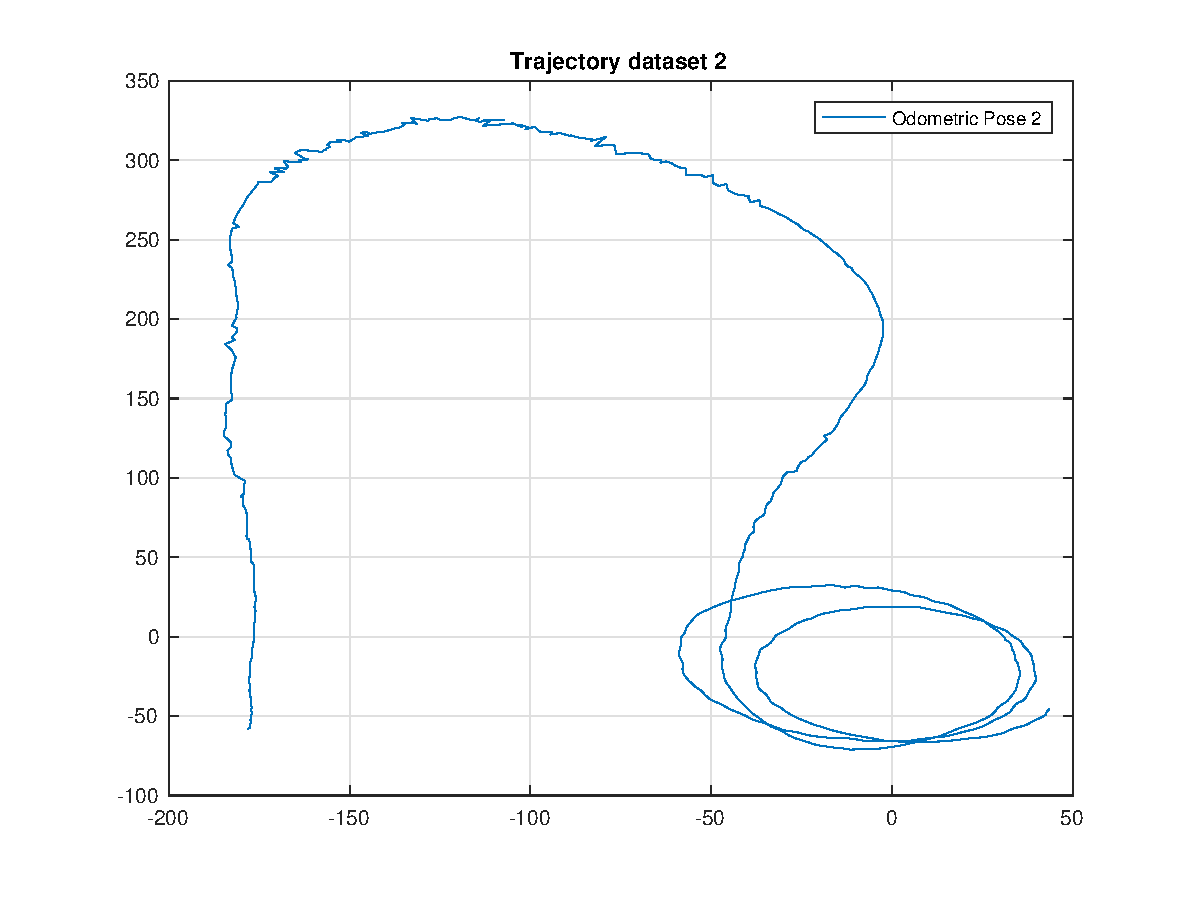
\includegraphics[width=.35\textwidth]{trajectory_dataset_2.eps}} \,
%\subfloat[][\emph{dataset 3}.]
%   {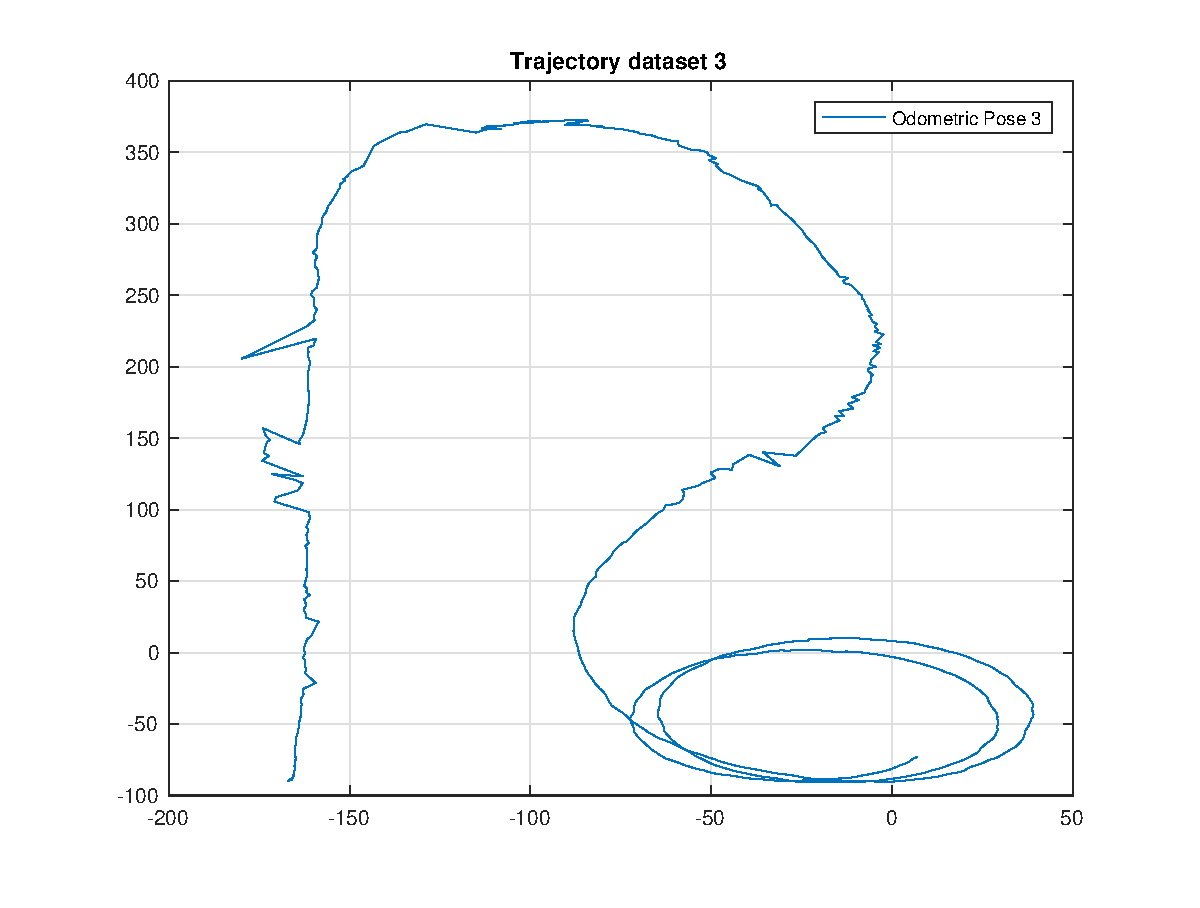
\includegraphics[width=.35\textwidth]{trajectory_dataset_3.eps}} \,
%\subfloat[][\emph{dataset 4}.]
%   {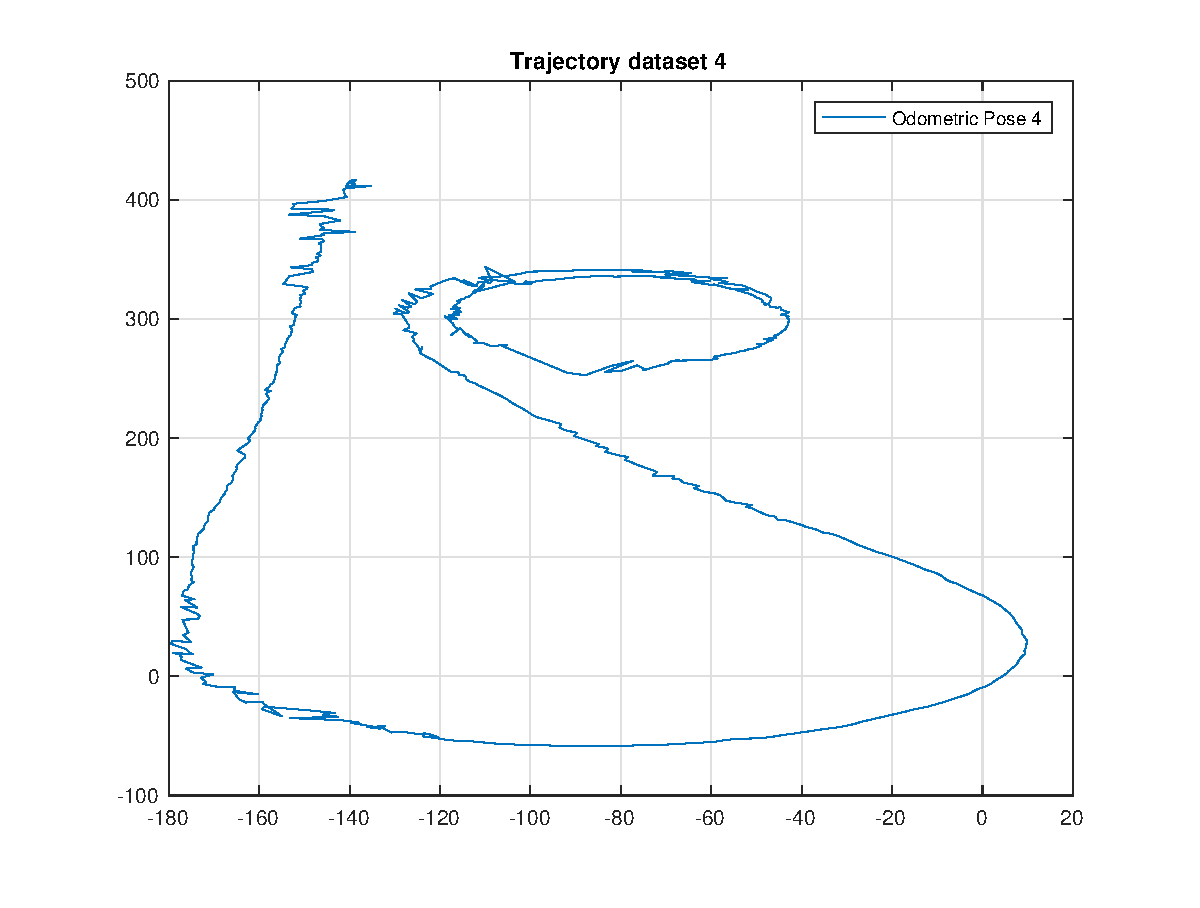
\includegraphics[width=.35\textwidth]{trajectory_dataset_4.eps}} \\
%\end{figure*}
%\begin{figure*}[htb]
%\subfloat[][\emph{dataset 1}.]
%   {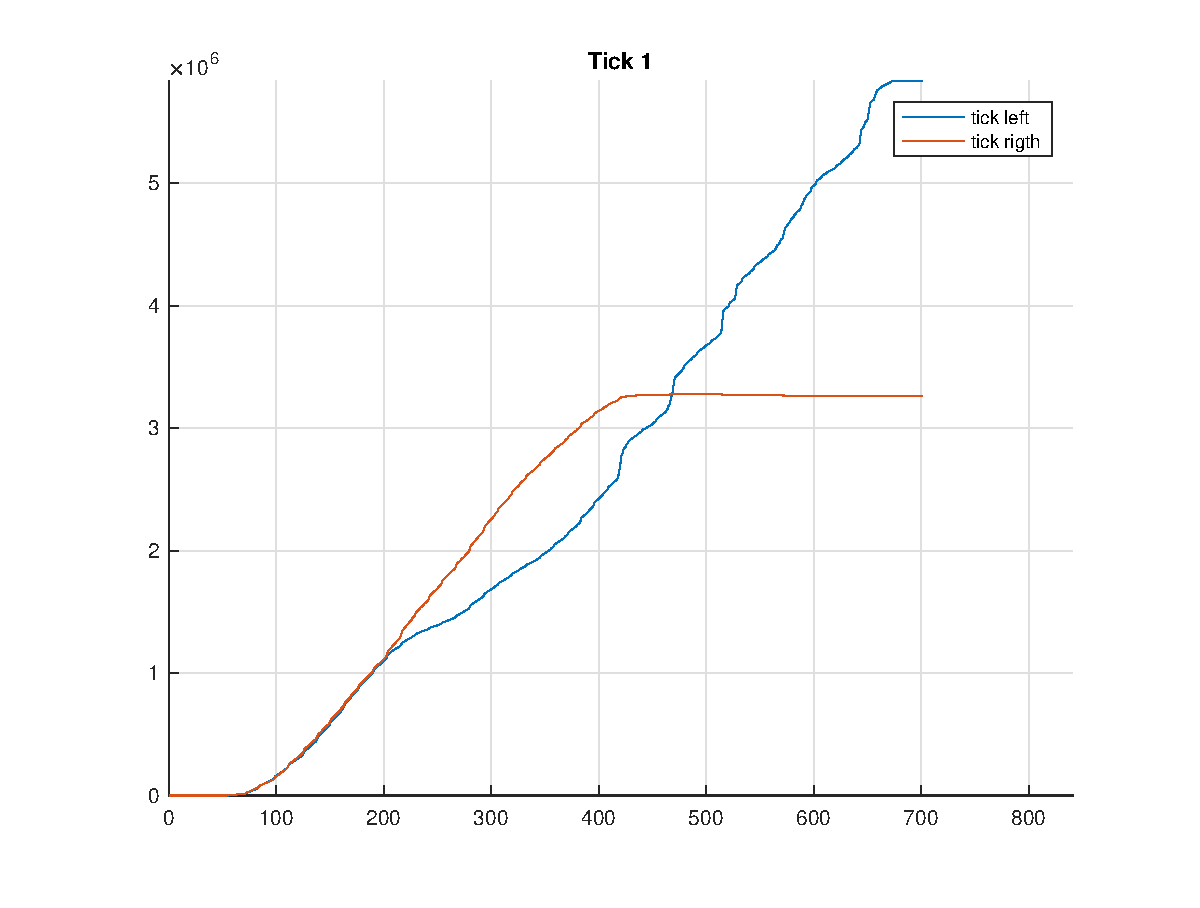
\includegraphics[width=.35\textwidth]{tick_dataset_1.eps}} \,
%\subfloat[][\emph{dataset 2}.]
%   {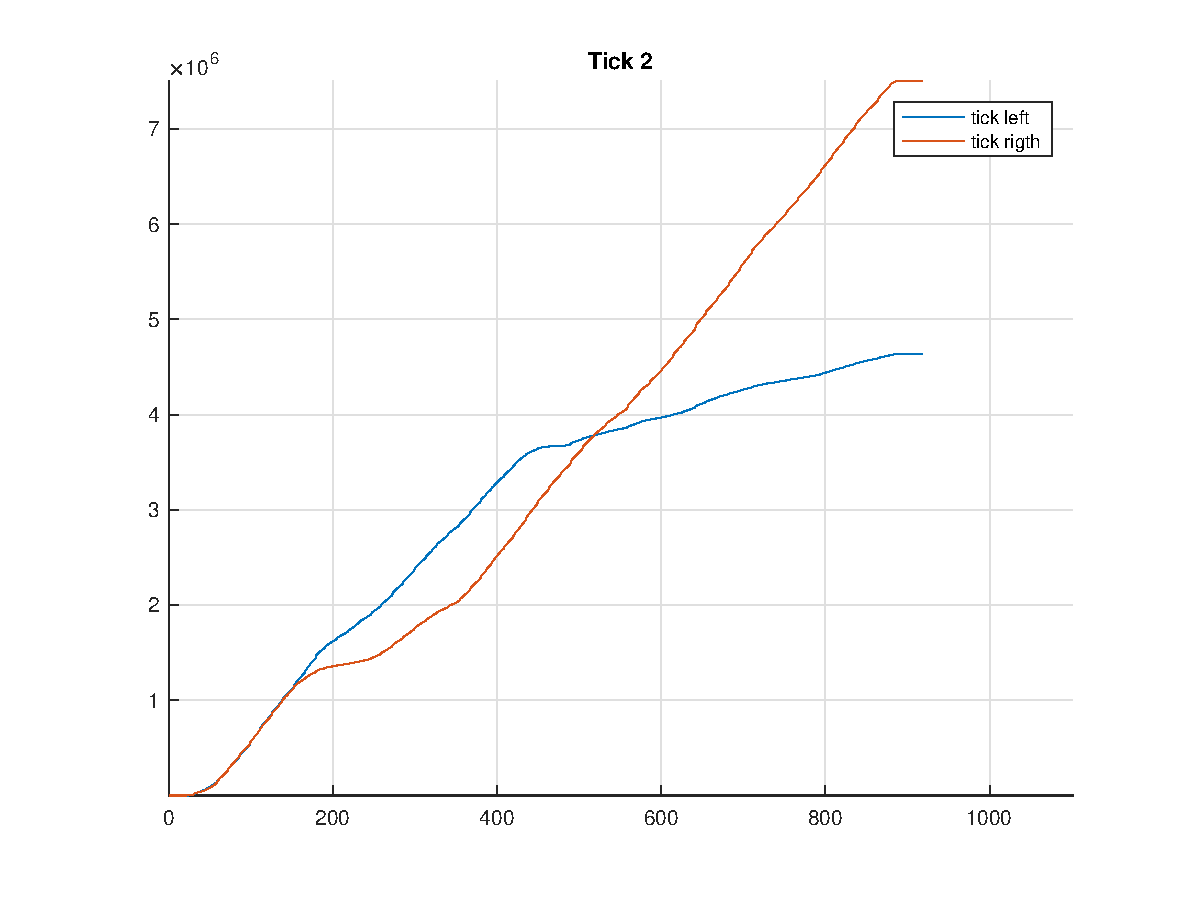
\includegraphics[width=.35\textwidth]{tick_dataset_2.eps}} \,
%\subfloat[][\emph{dataset 3}.]
%   {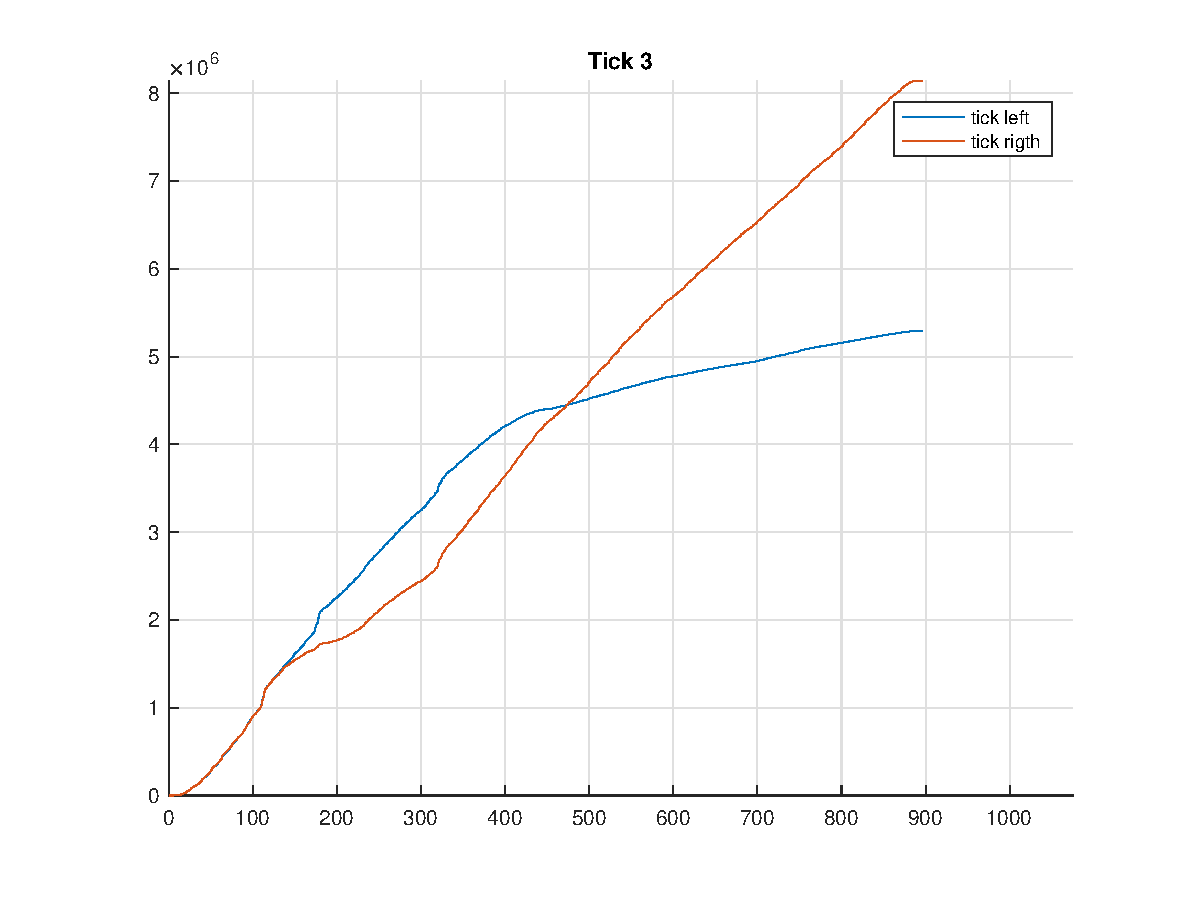
\includegraphics[width=.35\textwidth]{tick_dataset_3.eps}} \,
%\subfloat[][\emph{dataset 4}.]
%   {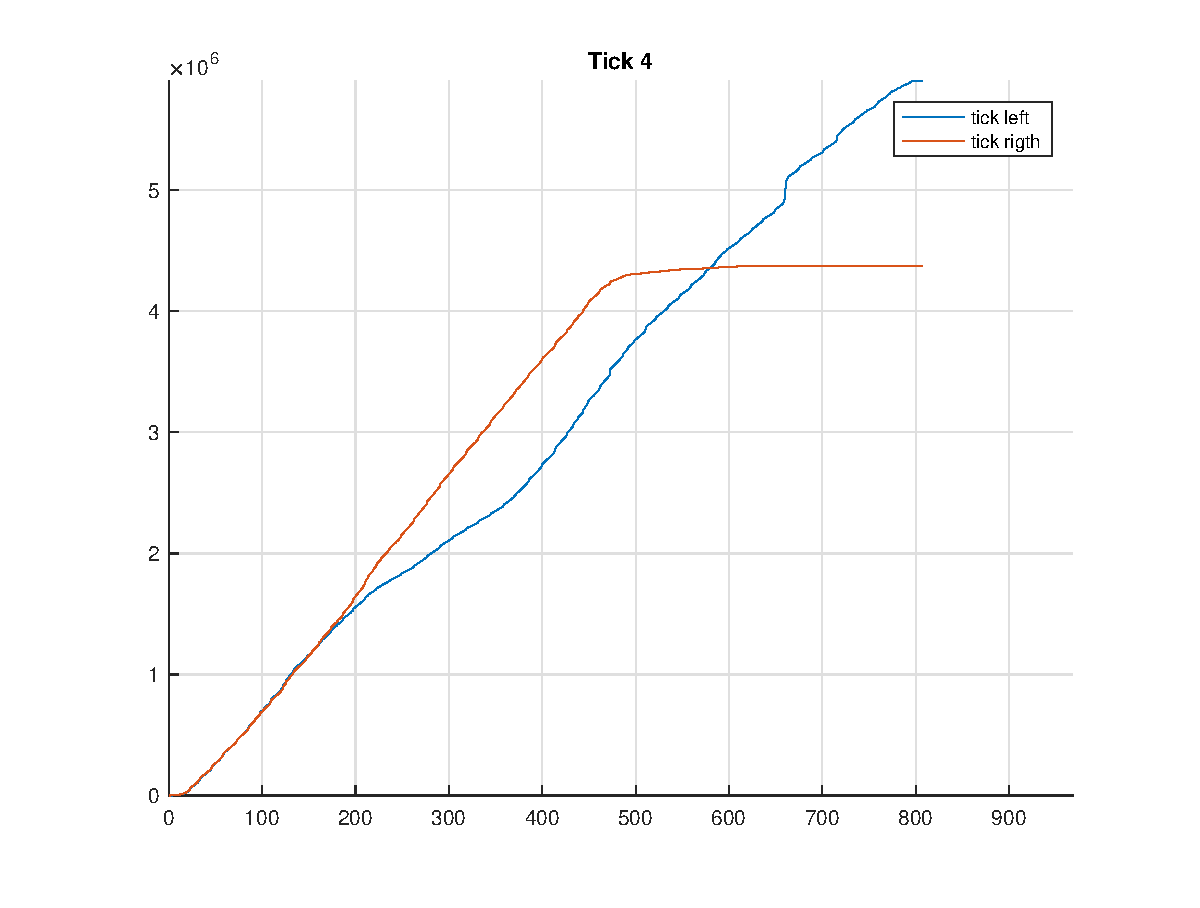
\includegraphics[width=.35\textwidth]{tick_dataset_4.eps}}
%\caption{Dataset}
%\label{fig:data}
%\end{figure*}
Finally, we show in the figures \ref{fig:OdoRec}, it shows the calculation for each path odometric with parameters previously estimated in comparison with the trajectory recorded by the camera.
\begin{figure*}[!ht]
\subfloat[][\emph{dataset 1}.]
   {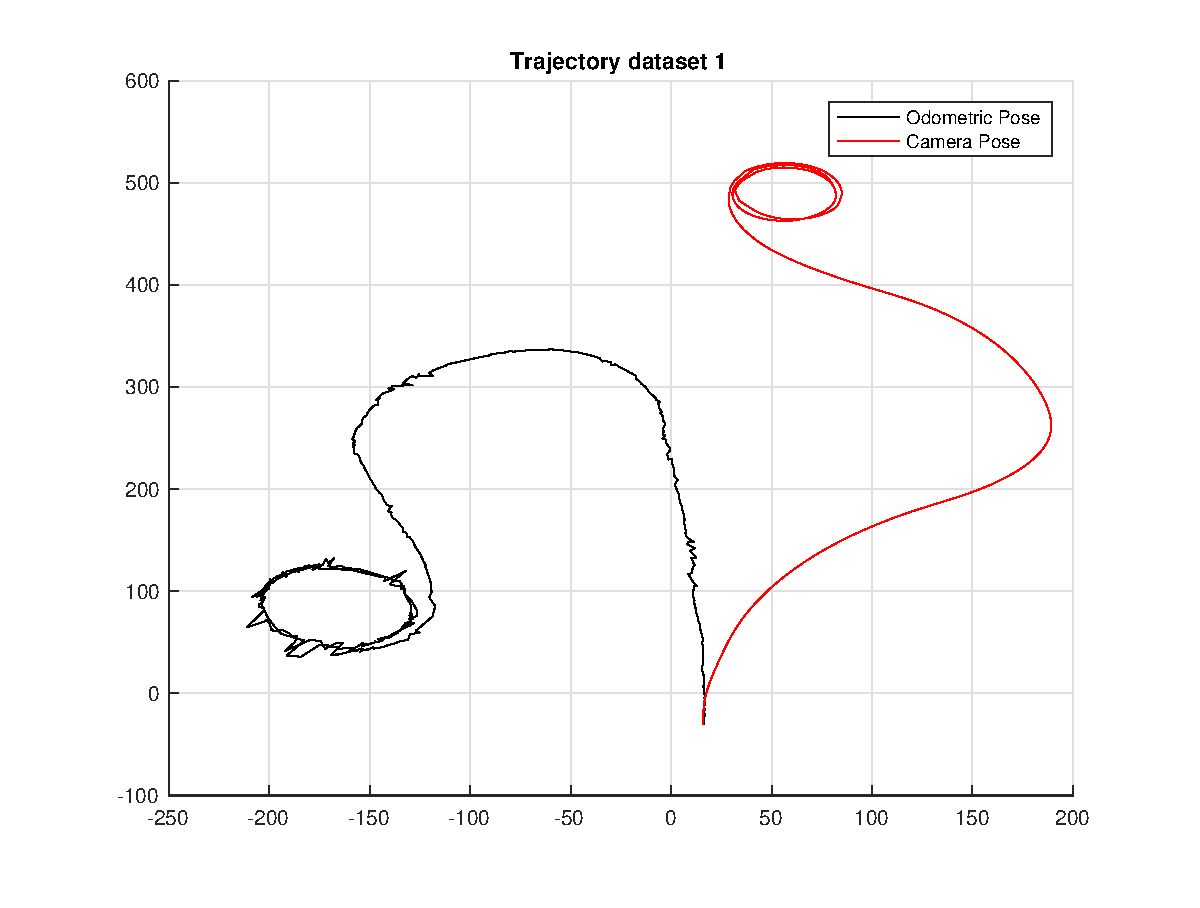
\includegraphics[width=0.5\textwidth]{odocam_1.eps}} \,
\subfloat[][\emph{dataset 2}.]
   {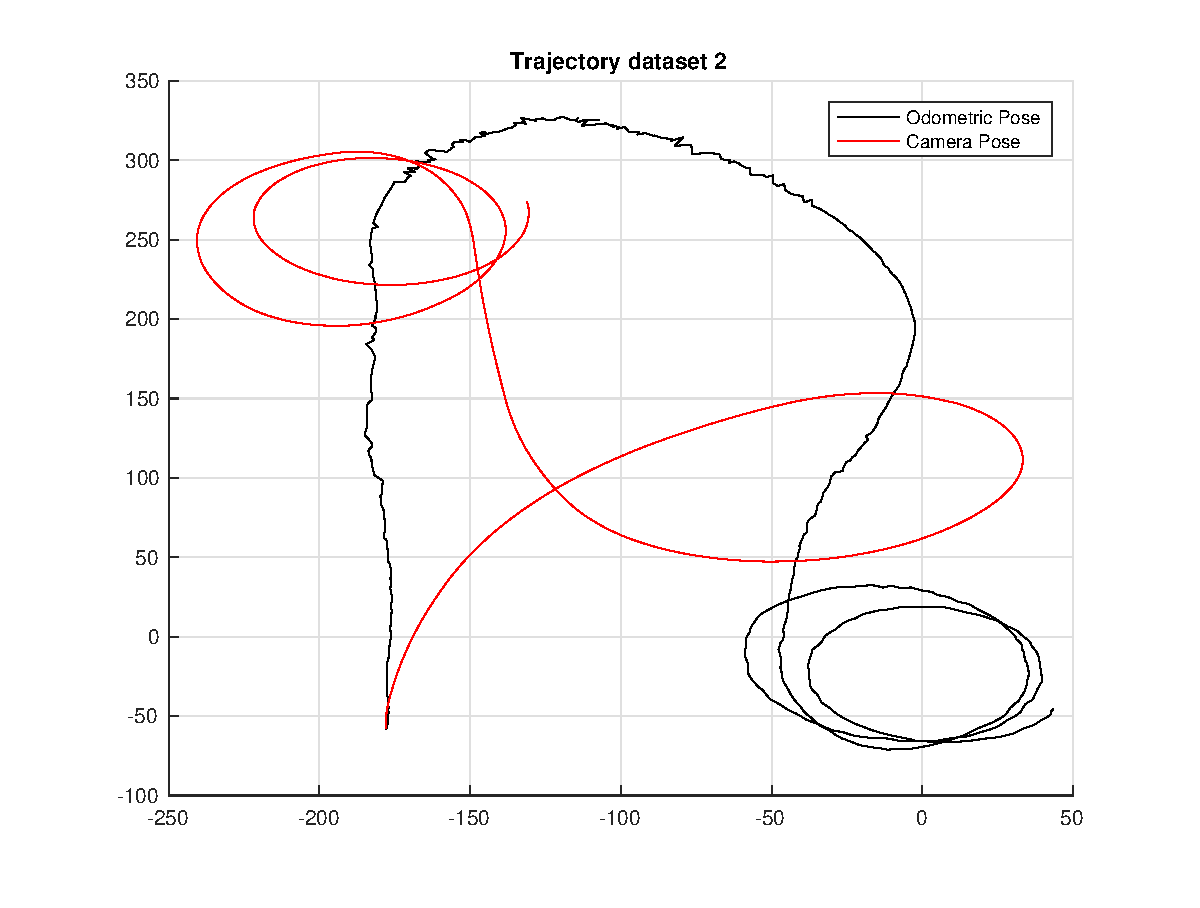
\includegraphics[width=0.5\textwidth]{odocam_2.eps}} \\
\subfloat[][\emph{dataset 3}.]
   {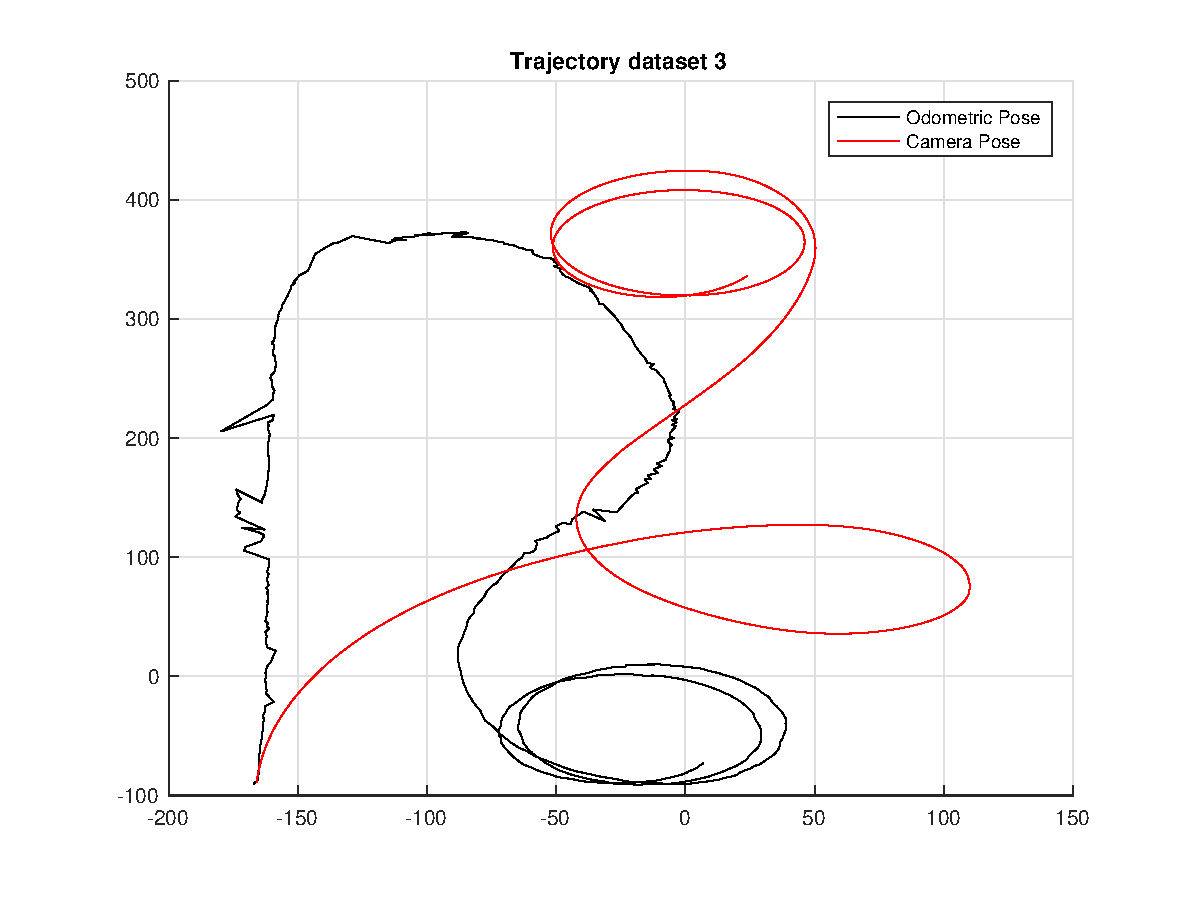
\includegraphics[width=0.5\textwidth]{odocam_3.eps}} \,
\subfloat[][\emph{dataset 4}.]
   {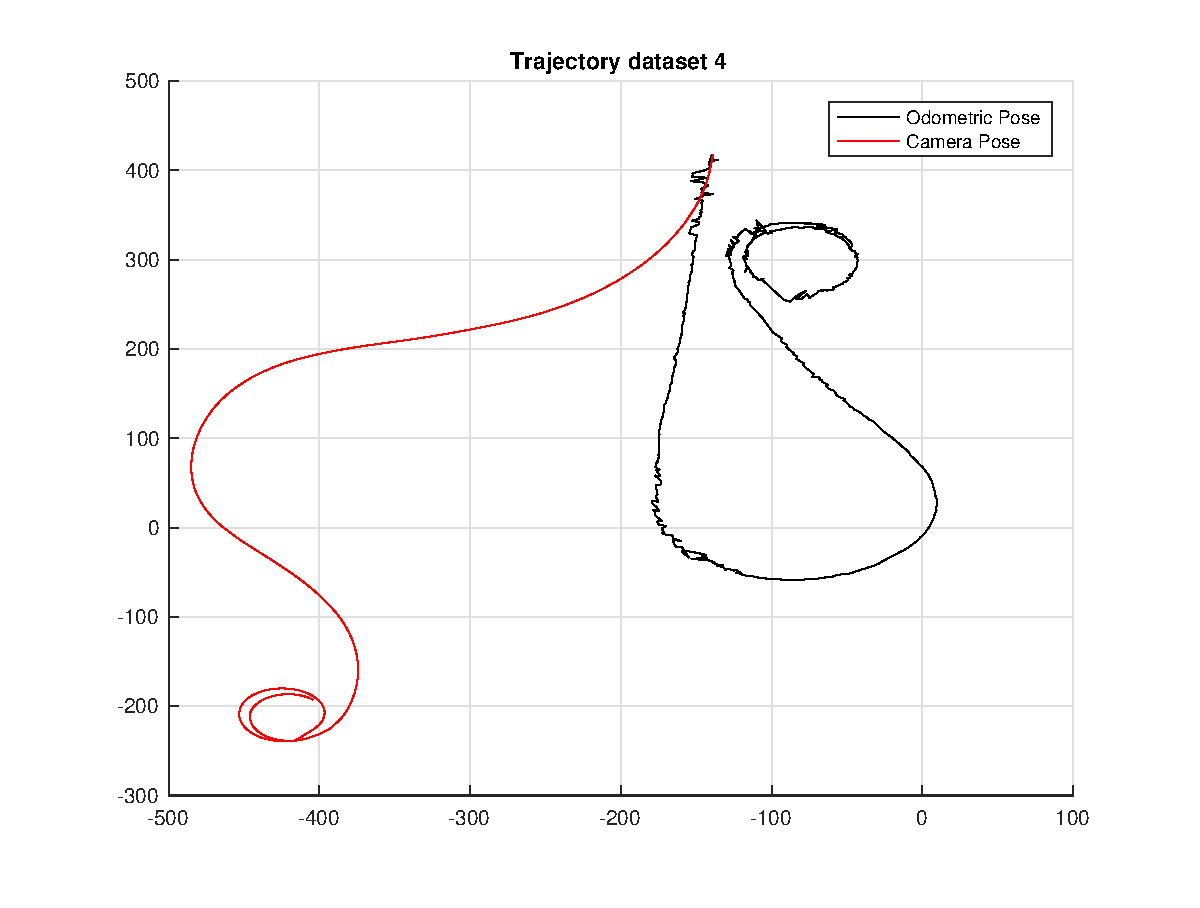
\includegraphics[width=0.5\textwidth]{odocam_4.eps}}
\caption{Odometry reconstruction}
\label{fig:OdoRec}
\end{figure*}